\documentclass[letterpaper]{article} 
\usepackage[margin=1in]{geometry}

%Set to 1 to compile Figures
\def\compileFigures{1}
\newcommand{\filename}{main}
\newcounter{figureNumber}

% !TeX root = ../main.tex
\PassOptionsToPackage{svgnames}{xcolor}
\usepackage{graphicx}
\usepackage{hyperref}

\usepackage{tcolorbox}
\tcbuselibrary{skins,breakable}
\usetikzlibrary{shadings,shadows}

\newenvironment{whyblock}[0]{%
	\tcolorbox[beamer,%
	noparskip,breakable,
	colback=LightGrey,colframe=DarkGrey,%
	colbacklower=LightGrey!75!DarkGrey,%
	title={\color{black} \large Why?}]}%
{\endtcolorbox}


\newenvironment{tipblock}[1]{%
	\tcolorbox[beamer,%
	noparskip,breakable,
	colback=LightGreen,colframe=DarkGreen,%
	colbacklower=LimeGreen!75!LightGreen,%
	title=#1]}%
{\endtcolorbox}
\newcommand{\why}{\paragraph{Why:}}


\title{Project template}

\begin{document}
\maketitle	

\begin{abstract}
This is a short guide to help you setup your latex projects. The guide also tries to provide reasons for why it is good to follow these guidelines, in form of Why-notes. If you're not interested in the reasons just skip over them.
\end{abstract}
\tableofcontents
%Main sections	
	% !TeX root = ../main.tex
\section{Project structure}\label{sec:projectStructure}

\begin{figure}
	\centering
	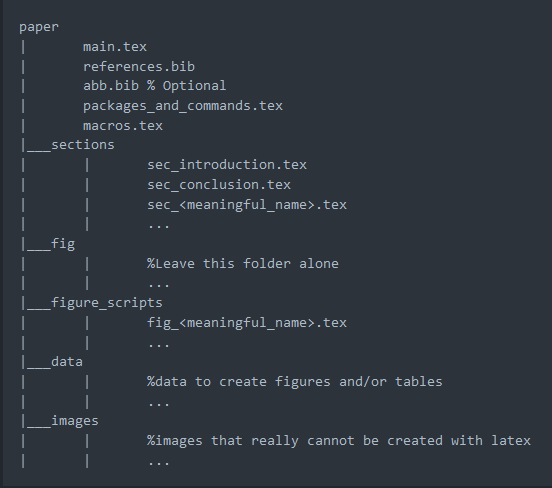
\includegraphics[width=\textwidth]{images/project_structure.png}
	\caption{The structure of the project.}
	\label{fig:projectStructure}
\end{figure}

\paragraph{Project structure}
Figure~\ref{fig:projectStructure} shows an overview of the project structure.

\why If everyone in the group follows the same structure it is easier to collaborate and you don't need to learn a new system all the time.

\paragraph{main.tex:} This is the main file of your document. Keep it as clean as possible. Conferences generally provide a template use this template to create the main file. Ideally only add the following in front of \verb|\begin{document}|:	
\verb|	|\\
\verb|	%Set to 1 to compile Figures|\\
\verb|	\def\compileFigures{0}|\\
\verb|	\newcommand{\filename}{main}|\\
\verb|	\newcounter{figureNumber}|\\
\verb|	|\\
\verb|	% !TeX root = ../main.tex
\PassOptionsToPackage{svgnames}{xcolor}
\usepackage{graphicx}
\usepackage{hyperref}

\usepackage{tcolorbox}
\tcbuselibrary{skins,breakable}
\usetikzlibrary{shadings,shadows}

\newenvironment{whyblock}[0]{%
	\tcolorbox[beamer,%
	noparskip,breakable,
	colback=LightGrey,colframe=DarkGrey,%
	colbacklower=LightGrey!75!DarkGrey,%
	title={\color{black} \large Why?}]}%
{\endtcolorbox}


\newenvironment{tipblock}[1]{%
	\tcolorbox[beamer,%
	noparskip,breakable,
	colback=LightGreen,colframe=DarkGreen,%
	colbacklower=LimeGreen!75!LightGreen,%
	title=#1]}%
{\endtcolorbox}|\\
\verb|	\newcommand{\why}{\paragraph{Why:}}|\\

	Don't write the sections in this file just use
	 \verb|\input{sections/sec_<section_name>}|.
	
	\why There will be multiple versions of your paper (submissions to different workshops, conferences, Arxiv, university events, etc.). Each requires a different template and you have to merge this template with your main.tex file. The simpler the main.tex file the better.
	
	\paragraph{package\_and\_commands.tex:} In this file you put all the \verb|\usepackage{}| imports and code for more complicated commands, which you might use in multiple projects.
	
	\why If you found a useful package or spent time creating a complicated command you want to reuse it.
	
	\paragraph{macros.tex:} This file contains all your project-specific macros. Use macros as much as possible. For example, instead of writing \verb|\mathbb{R}| every time for the real numbers create a macro \verb|\newcommand{\R}{\mathbb{R}}|. Create macros when referring to existing algorithms, data sets, and names of things. When you go through your files with Ctrl + f trying to change every instance of a declaration you decided to change the notation for, you should have created a macro for that.
	
	Why: Macros are often project specific having all of them in a small file makes it easier for collaborators to find them.
	
	\paragraph{references.bib:} The file containing all your citation references. See in the Citations section on how to create the citations.
	
	\why Keep the main.tex file clean.
	
	\paragraph{sections:} Each section of your paper should be in a separate .tex-file in this folder, give them meaningful names that start with \verb|sec_|.
	
	\why This simplifies the main file and makes it easier for people to work on different sections simultaneously.
	
	\paragraph{fig:} The figures generated by your scripts will be saved in this folder. Add everything but the .pdf-files to .gitignore.
	
	\why Compiling figures can get time-consuming and sometimes requires specific settings. People not working on the figures can just input them as .pdf See Figures for more information.
	
	\paragraph{figure\_scripts:} Each figure you create with TikZ or PGFPlots should be in a separate file with a meaningful name in this folder (starting with \verb|fig_|).
	
	\why The code to generate figures can get long and make it harder to work on the text. Outsourcing the scripts makes the files cleaner.
	
	\paragraph{data:} The data used in your graphics.
	
	\why When you rerun some experiment you only need to replace the data.
	
	\paragraph{images:} This folder contains images (e.g. .png, .jpg.) that are used in the paper. It should not contain graphics you generated somewhere else, but really only pictures.
	
	Why: Keep the main folder clean.
	

	% !TeX root = ../main.tex
\section{Naming conventions and references}\label{sec:namingConventions}
Give everything meaningful names and create labels \verb|\label{<name>}| for sections, figures, and tables as soon as you create them.

Use \texttt{sec:<meaningfulname>} , \texttt{fig:<meaningfulname>} , \texttt{tab:<meaningfulname>}, \texttt{eq:<meaningfulname>} when creating labels for sections, figures, tables and equations respectively.

A meaningful name is a name that tells the reader (i.e. future you or a collaborator) what the label refers to. For sections the section title is a good start. Avoid using numbers and cryptic letter combinations.

\begin{whyblock} You want others and future you to be able to understand what the label means.\end{whyblock}


	\section{Citations}\label{sec:citations}

When you want to create a new reference. Use the bibtex entries provided by Google Scholar.

\begin{enumerate}
	\item Go to \href{https://scholar.google.com/}{Google Scholar}.
\item Search for the paper.
\item Go on All <versions> and find the right version (i.e. where possible the final conference/journal version)
\item Click on cite ()
\item Click on BibTeX and copy the entry
\item Double-check and fix the entry if something is wrong.
\end{enumerate}

If you have to create a bibtex entry from scratch (because it doesn't exist on Google Scholar), follow the reference format \verb|<lastname_first_author><yyyy><first_proper_word_title>|.

\begin{whyblock}
 Everyone following one convention avoids duplicate citations. GoogleScholar has an easy format and is a good start for almost any bibtex entry.
\end{whyblock}

\textbf{Optional:} If you want consistent references to a venue you can use the abb.bib file. Change the booktitle to \verb|booktitle=proc # {<xx>th} # <venue_name>|

\textbf{Tip:} There is a Google Scholar browser extension that creates a button to directly search.
	\section{Figures}\label{sec:figures}
There are two wonderful packages in LaTeX to create figures TikZ and PGFPlots. The former can be used to create any kind of vector graphic, the latter focuses on plots. Together they can create almost any kind of figure you need for a paper. Use them.

\begin{whyblock}

\begin{itemize}

\item Creating figures inside LaTeX ensures that they use the correct font. You can scale the figure without ending up with tiny fonts.
\item They just look better.
\item Makes it easier to switch between different templates, often a simple change to the scale of the figure is enough. Externally created figures are harder to scale when desiring consistent font(size).
\end{itemize}
\end{whyblock}
When using figures, put the following statement into your main.tex file before
 \verb|% !TeX root = ../main.tex
\PassOptionsToPackage{svgnames}{xcolor}
\usepackage{graphicx}
\usepackage{hyperref}

\usepackage{tcolorbox}
\tcbuselibrary{skins,breakable}
\usetikzlibrary{shadings,shadows}

\newenvironment{whyblock}[0]{%
	\tcolorbox[beamer,%
	noparskip,breakable,
	colback=LightGrey,colframe=DarkGrey,%
	colbacklower=LightGrey!75!DarkGrey,%
	title={\color{black} \large Why?}]}%
{\endtcolorbox}


\newenvironment{tipblock}[1]{%
	\tcolorbox[beamer,%
	noparskip,breakable,
	colback=LightGreen,colframe=DarkGreen,%
	colbacklower=LimeGreen!75!LightGreen,%
	title=#1]}%
{\endtcolorbox}|:

\verb|%Set to 1 to compile Figures|\\
\verb|\def\compileFigures{0}|\\
\verb|\newcommand{\filename}{main}|\\
\verb|\newcounter{figureNumber}|\\

Your \verb|packages_and_commands.tex\verb| file should contain:

\verb|\usepackage{tikz}|\\
\verb|\if\compileFigures1|\\
\verb|\usetikzlibrary{external}|\\
\verb|\tikzexternalize[prefix=fig/] % activate!|\\
\verb|\fi|

Important: To use the external library you need to add -shell-escape to your compile command. How to do this depends on your IDE.

For every figure you create use the following template:

\verb|\begin{figure}|\\
\verb|	\centering|\\
\verb|	\if\compileFigures1|\\
\verb|	\input{figure_scripts/fig_<meaningful_filename>}|\\
\verb|	\else|\\
\verb|	\includegraphics[]{fig/\filename-figure\thefigureNumber.pdf}|\\
\verb|	\stepcounter{figureNumber}|\\
\verb|	\fi|\\
\verb|	\caption{<meaningful_caption>}|\\
\verb|	\label{fig:<meaningful_label>}|\\
\verb|\end{figure}|

\begin{whyblock}
\begin{itemize}
\item With this setup, by changing \verb|\def\compileFigures{0}| you can switch from creating the figures to just including them as pre-generated pdfs.
\item For the camera ready version of your paper you submit your code. Here you want to ensure that everything compiles correctly, this is easier when just submitting the .pdf of each figure.
\item Allows a collaborator to compile the file without compiling the figures.
\end{itemize}
\end{whyblock}

\textbf{Note:} If your figure consists of <x> Tikz pictures, the two lines in the \verb|\else| block need to be repeated <x> times.

\textbf{Tip:} If you have multiple figures with a common legend you can use the following code to create the legend:

\verb|\begin{tikzpicture}|\\
\verb|	\begin{axis}[scale=0.01,|\\
\verb|		hide axis,|\\
\verb|		xmin=0, xmax=1,|\\
\verb|		ymin=0, ymax=1,|\\
\verb|		legend columns=<number>,|\\
\verb|		]|\\
\verb|		\addlegendimage{<configuration_of_entry>}|\\
\verb|		\addlegendentry{<name>};|\\
\verb|		%Example|\\
\verb|		\addlegendimage{blue,mark=square*}|\\
\verb|		\addlegendentry{QII};|\\
\verb|	\end{axis}|\\
\verb|\end{tikzpicture}|
	\section{Tables}\label{sec:tables}
	\section{Generating diff files}\label{sec:diffFiles}
\begin{enumerate}
\item If you want to generate diff file for two folders (e.g., one folder has updated version and one folder has the old version), you can use the diff.sh in this folder to do so. It requires three inputs: old folder, new folder and output folder. The script loops all tex files in the sections folder and root folder to compute the diff between the file in the older folder and the one in the new folder with the same file name and output the file into the output folder. Besides, the script copies files in other folders (e.g., image, figure\_scripts) to the output folder. After the execution, you can compile files in the output folder to get diff file. Example: \verb|bash diff.sh submitted_version new_version diff|

\item Instead, if you want to generate diff file between two commits on Github, things become easier.
\end{enumerate}
\begin{itemize}
\item Install latexdiff first. Check instructions for Ubuntu, Windows and MacOS.
\item Install git-latexdiff. Check instructions here.
\item Run the following commands based on your needs: Diff the previous revision with the latest commit:
\end{itemize}

\verb|git latexdiff HEAD^ --main main.tex|

Diff the latest commit with the working tree:

\verb|git latexdiff HEAD -- --main main.tex|

Diff latest commit with branch master:

\verb|gt latexdiff master HEAD --main main.tex|

Pass --type=CHANGEBAR to latexdiff to get changebars in the margins instead of red+trike/blue+underline diff:

\verb|git latexdiff --type=CHANGEBAR HEAD^ --main main.tex|

Use a specific latexdiff configuration file:

\verb|git latexdiff --config /path/to/file HEAD^ --main main.tex|

Note that, for those two versions, you should set compileFigures to 0. The diff will not highlight the changes of figures inside the tikzpicture but will highlight changes in the captions. In addition, you need to generate bbl manually (by runing bibtex main.tex) for these two versions and \verb|run git latexdiff HEAD^ --main main.tex ----flatten| if you want to see the changes in the reference.bib.
	\section{Useful Tools}\label{sec:usefulTools}

	
%Bibliography
\bibliography{references}

\end{document}